\documentclass[journal]{IEEEtran}

% ===================
% Packages
% ===================
\usepackage[utf8]{inputenc}
\usepackage[T1]{fontenc}
\usepackage{lmodern}
\usepackage[spanish]{babel}
\usepackage{amsmath, amsfonts, amssymb}
\usepackage{graphicx}
\usepackage{cite}
\usepackage{xcolor}
\usepackage{array}
\usepackage{multirow}
\usepackage[hyphens]{url}
\usepackage{subfig}
\usepackage{tikz}
\usetikzlibrary{babel,arrows.meta,positioning,fit}
\usepackage{booktabs}
\usepackage{algorithm}
\usepackage{algorithmic}
\usepackage[breaklinks=true,hidelinks]{hyperref}

% Bloque de "pendiente" bien visible en el PDF compilado, para las
% secciones que dependen del trabajo estadistico de la extension todavia
% en curso -- se reemplaza por contenido real antes de la entrega.
\newcommand{\pendiente}[1]{%
  \begin{quote}\small\color{black!60}%
  \textbf{[PENDIENTE --- #1]}
  \end{quote}%
}

% ===================
% Title and Authors
% ===================
\title{Planificador por Lotería en Espacio de Usuario:\\
Diseño, Verificación y Extensión con \textit{Compensation Tickets}}

\author{
    Isaac Francisco Moreno Fuentes,~\\
    Emmanuel Barrantes Vargas\\
    \thanks{Isaac Francisco Moreno Fuentes y Emmanuel Barrantes Vargas son estudiantes del curso MC 6004 Sistemas Operativos Avanzados, Tecnológico de Costa Rica, II semestre 2026.}
}

% ===================
% Beginning of Document
% ===================
\begin{document}
\maketitle

\begin{abstract}
Este informe documenta el diseño, la implementación y la verificación de un
planificador de CPU por lotería (\textit{lottery scheduling}) en espacio de
usuario, inspirado en el trabajo de Waldspurger y Weihl~\cite{Waldspurger1994}.
El sistema coordina tareas concurrentes mediante \textit{pthreads}, un mutex
y variables de condición, sin espera activa ni un único bloqueo que impida
demostrar el protocolo de despacho. Los siete casos mínimos de
funcionamiento exigidos cumplen sin hallazgos bajo los \textit{sanitizers}
requeridos, y el experimento de proporcionalidad confirma que el sorteo
pondera correctamente por boletos, con un error absoluto medio muy por
debajo de la tolerancia del enunciado. La extensión elegida,
\textit{compensation tickets}, se valida con un experimento A/B propio: la
tarea que cede tempranamente y recibe boletos compensados recupera una
participación de CPU sustancialmente más cercana a su valor objetivo
(mejora relativa de $+63.7\%$, estadísticamente significativa). El informe
cierra con una comparación conceptual contra el paper original y una
discusión crítica de los \textit{trade-offs} de diseño más relevantes.
\end{abstract}

\begin{IEEEkeywords}
lottery scheduling, proportional-share, pthreads, sincronización, compensation tickets
\end{IEEEkeywords}

% ===================
% Main Sections
% ===================
\section{Introducción}

La planificación por lotería (\textit{lottery scheduling}) representa
derechos de uso del CPU mediante boletos: en cada decisión de despacho se
sortea un boleto al azar entre las tareas activas y la propietaria del
boleto ganador recibe el siguiente intervalo de ejecución. A largo plazo, si
la selección es uniforme, la fracción de CPU que recibe una tarea converge a
su fracción de los boletos activos --- la propiedad de \textit{proportional
share} que motiva el mecanismo, descrita originalmente por Waldspurger y
Weihl~\cite{Waldspurger1994}.

Este proyecto traduce esa política a un mecanismo ejecutable y verificable:
un planificador en espacio de usuario, escrito en C17 sobre \textit{pthreads}
POSIX, que no modifica el \textit{kernel} ni sustituye el planificador de
GNU/Linux. El programa simula la existencia de un único CPU lógico ---cada
tarea es un hilo que solo avanza su trabajo cuando el planificador se lo
permite explícitamente--- y usa como carga de trabajo instrumentada el
cálculo incremental de la serie de Taylor de $\arcsin(1) = \pi/2$, elegida
por tener estado real que preservar entre activaciones (término anterior,
suma acumulada, índice) y por ser verificable contra un valor conocido.

\subsection{Alcance de este informe}

Las secciones siguientes cubren, en orden: la arquitectura del sistema y el
protocolo de sincronización (datos compartidos, mutex, variables de
condición y sus predicados de espera); el pseudocódigo de los algoritmos
centrales del sorteo, la activación, la cesión y la terminación; la
verificación contra los siete casos mínimos de funcionamiento que exige el
enunciado, incluyendo la evidencia de \textit{sanitizers}; los resultados del
experimento de proporcionalidad; el diseño e implementación de la extensión
elegida (\textit{compensation tickets}); un análisis comparativo con el paper
original de Waldspurger y Weihl, incluyendo las diferencias con su prototipo
sobre Mach 3.0 y las limitaciones de este prototipo en espacio de usuario; y
una discusión de los \textit{trade-offs} de diseño más relevantes. El código
fuente completo, la trazabilidad del equipo y el historial de decisiones de
diseño extendido viven en los repositorios públicos del proyecto, citados
donde corresponde.

\section{Arquitectura y Protocolo de Sincronización}
\label{sec:arquitectura}

\subsection{Modelo de hilos}

El hilo principal (\texttt{main()}) actúa como el planificador; no existe un
hilo dedicado separado para esta responsabilidad. El programa simula un
único CPU lógico, por lo que no hay razón para que el planificador sea una
entidad concurrente distinta del programa que lo invoca: esta decisión
reduce en uno el número de hilos a crear, sincronizar y unir, y simplifica el
argumento de terminación. Además del hilo principal, se crea un
\texttt{pthread} por tarea (entre 5 y 25), cada uno ejecutando
\texttt{worker\_thread\_main}. Todo hilo creado se une con
\texttt{pthread\_join} antes de que el programa termine.

\subsection{Datos compartidos}

Dos estructuras concentran todo el estado que más de un hilo puede tocar:

\begin{itemize}
\item \textbf{\texttt{Task}} (una por tarea): identificador, boletos base
  (\texttt{tickets}), boletos efectivos (\texttt{effective\_tickets}, igual a
  \texttt{tickets} salvo compensación activa, Sección~\ref{sec:extension}),
  estado (\texttt{READY}/\texttt{RUNNING}/\texttt{FINISHED}), trabajo total y
  ejecutado, contador de despachos, estado privado de la serie de $\pi$, y su
  propia variable de condición \texttt{cond\_worker}.
\item \textbf{\texttt{Sync}} (una para todo el programa): un
  \texttt{pthread\_mutex\_t}, la variable de condición
  \texttt{cond\_scheduler} que espera el planificador, su predicado
  \texttt{event\_ready}, y la bandera \texttt{stop\_requested} que activa
  \texttt{--max-dispatches}.
\end{itemize}

Un único mutex (\texttt{sync.mutex}) protege el estado de todas las
\texttt{Task} (\texttt{state}, \texttt{dispatch\_count},
\texttt{effective\_tickets}, \texttt{debt}), \texttt{event\_ready} y
\texttt{stop\_requested}. Ese mutex \textbf{no} envuelve la ejecución de las
unidades de trabajo de $\pi$: hacerlo violaría la prohibición explícita del
enunciado de proteger toda la ejecución con un único bloqueo, y además sería
innecesario. La Sección~\ref{sec:invariante} explica por qué omitirlo ahí es
seguro.

\subsection{Variables de condición y predicados de espera}

Se usa un esquema de \textbf{una \texttt{cond\_worker} por tarea más una
\texttt{cond\_scheduler} compartida}, en vez de una única condvar global con
un predicado de ``turno'' señalada por \textit{broadcast}. La alternativa
descartada despertaría innecesariamente a las $N-1$ tareas que no ganaron
cada despacho --- el problema de \textit{thundering herd}: muchos hilos
despertados por un mismo evento cuando a lo sumo uno puede hacer trabajo
útil, desperdiciando ciclos de CPU y generando contención de mutex
innecesaria en los demás~\cite{MolloyLever2000}. El esquema elegido lo
evita señalando siempre de forma dirigida
(\texttt{pthread\_cond\_signal}, nunca \texttt{pthread\_cond\_broadcast}) a
un único hilo por evento. La Tabla~\ref{tab:condvars} resume las dos
condvars del protocolo: quién espera en cada una, su predicado exacto, y
quién la señala.

\begin{table*}[htbp]
\caption{Condvars, predicados y quién señala}
\label{tab:condvars}
\centering
\renewcommand{\arraystretch}{1.4}
\begin{tabular}{p{3.0cm}p{2.6cm}p{4.5cm}p{7.0cm}}
\toprule
\textbf{Condvar} & \textbf{Espera} & \textbf{Predicado} & \textbf{Señala} \\
\midrule
\texttt{task[i].cond\_worker} &
  Worker $i$ &
  \texttt{state==RUNNING || stop\_requested} &
  El planificador, al elegir a $i$ como ganador (o \texttt{sync\_request\_stop} al cortar) \\
\midrule
\texttt{cond\_scheduler} &
  El planificador &
  \texttt{event\_ready} &
  El worker en ejecución, al ceder o terminar \\
\bottomrule
\end{tabular}
\end{table*}

Ambos predicados se evalúan dentro de un \texttt{while}, nunca un
\texttt{if}, por dos razones independientes: POSIX permite explícitamente
que \texttt{pthread\_cond\_wait} retorne sin que nadie haya señalado la
condición~\cite{IEEE1003.1-2024} --- un despertar sin causa aparente,
conocido en la literatura de \textit{pthreads} como \textit{spurious
wakeup}~\cite{Butenhof1997}; y el caso en que varios hilos comparten una
condvar y el que despierta encuentra que la condición ya no aplica. \texttt{pthread\_cond\_wait} suelta el mutex y duerme el hilo de
forma atómica, y vuelve a tomar el mutex antes de retornar --- evita la
condición de \textit{señal perdida} que ocurriría si soltar el mutex y
dormirse fueran dos pasos separados.

\subsection{Protocolo de despacho}
\label{sec:protocolo}

La Fig.~\ref{fig:protocolo} muestra el ciclo completo de un despacho (el
pseudocódigo correspondiente es el Algoritmo~\ref{alg:bucle},
Sección~\ref{sec:algoritmos}). El planificador (hilo principal) ejecuta
tres pasos en secuencia:
\texttt{sync\_select\_winner} (sortea la ganadora entre las tareas
\texttt{READY}, ponderando por \texttt{effective\_tickets}),
\texttt{sync\_dispatch} (marca a la ganadora \texttt{RUNNING} y la señala), y
\texttt{sync\_wait\_for\_event} (se bloquea hasta que esa tarea ceda o
termine). El worker ganador, mientras tanto, estaba bloqueado en
\texttt{sync\_wait\_for\_dispatch}; al despertar, ejecuta su porción de
trabajo \textbf{fuera del mutex} y cierra el ciclo con
\texttt{sync\_finish\_turn}, que actualiza su estado y despierta al
planificador.

\begin{figure}[htbp]
\centering
\begin{tikzpicture}[
    box/.style={draw=black, rounded corners=3pt, text width=3.65cm,
                minimum height=0.9cm, align=center, font=\scriptsize},
    arr/.style={-{Stealth[length=2mm]}, thick},
    lbl/.style={font=\tiny, align=center},
    node distance=6mm
]
\node[box, fill=blue!8] (sel) {\texttt{sync\_select\_winner}\\(toma mutex, suma \texttt{effective\_tickets} de READY, sortea, suelta mutex)};
\node[box, fill=blue!8, below=of sel] (disp) {\texttt{sync\_dispatch}\\(toma mutex, assert exclusión, \texttt{state=RUNNING}, \texttt{signal(cond\_worker[i])}, suelta mutex)};
\node[box, fill=blue!8, below=of disp] (wait) {\texttt{sync\_wait\_for\_event}\\(toma mutex, \texttt{while(!event\_ready) cond\_wait}, suelta mutex)};

\node[box, fill=orange!12, below=16mm of wait] (wd) {\texttt{sync\_wait\_for\_dispatch}\\(worker $i$, dormido hasta \texttt{state==RUNNING})};
\node[box, fill=green!12, below=of wd] (work) {\texttt{workload\_run\_units}\\ \textbf{(sin mutex)} --- seguro por el invariante de exclusión};
\node[box, fill=orange!12, below=of work] (fin) {\texttt{sync\_finish\_turn}\\(toma mutex, \texttt{state=READY|FINISHED}, \texttt{event\_ready=1}, \texttt{signal(cond\_scheduler)}, suelta mutex)};

\draw[arr] (sel.south) -- (disp.north);
\draw[arr] (disp.south) -- (wait.north);
\draw[arr] (disp.east) to[out=-20,in=90] node[lbl, right=1pt] {signal\\dirigida} (wd.north east);
\draw[arr] (wd.south) -- (work.north);
\draw[arr] (work.south) -- (fin.north);
\draw[arr] (fin.west) to[out=160,in=-90] node[lbl, left=1pt] {signal} (wait.south west);
\draw[arr, dashed] (fin.east) to[out=20,in=-90] node[lbl, right=1pt] {si READY,\\vuelve a\\esperar} (wd.south east);
\end{tikzpicture}
\caption{Un ciclo de despacho. Las cajas azules corren en el hilo
planificador (\texttt{main}); las naranjas y la verde, en el hilo worker de
la tarea ganadora. Solo el tramo verde corre sin el mutex tomado.}
\label{fig:protocolo}
\end{figure}

\subsection{Por qué es seguro ejecutar el trabajo sin el mutex}
\label{sec:invariante}

El invariante de exclusión --- como máximo una tarea en \texttt{RUNNING} en
todo momento, garantizado por el \texttt{assert} dentro de
\texttt{sync\_dispatch} --- implica que mientras una tarea corre, ningún
otro hilo lee ni escribe sus campos: el planificador está bloqueado en
\texttt{sync\_wait\_for\_event} (no toca ninguna \texttt{Task}), y los demás
workers están bloqueados en \texttt{sync\_wait\_for\_dispatch} esperando su
propia señal (nunca tocan una tarea ajena). El único hilo que puede tocar la
tarea mientras corre es su propio dueño. Esta es una invariante del
\emph{protocolo} (el orden de llamadas), no algo que un \textit{sanitizer}
pueda verificar por sí solo --- de ahí que cualquier código nuevo que
necesite leer el progreso de una tarea \texttt{RUNNING} desde otro hilo (por
ejemplo, un log en vivo) deba traer esa lectura dentro del mutex
explícitamente, en vez de asumir que es seguro por analogía con este caso.

\subsection{Terminación limpia y \texttt{--max-dispatches}}

El enunciado exige que ningún trabajador quede bloqueado al finalizar. Una
tarea que llega a \texttt{FINISHED} simplemente retorna de
\texttt{worker\_thread\_main}. El caso menos obvio es
\texttt{--max-dispatches}: cuando el planificador alcanza el límite, una
tarea todavía \texttt{READY} que nunca vuelve a ser elegida se quedaría
esperando su señal para siempre. \texttt{sync\_request\_stop} resuelve esto
señalando la \texttt{cond\_worker} de cada tarea \texttt{READY} sin cambiar
su estado; \texttt{sync\_wait\_for\_dispatch} retorna un código distinto de
cero en ese caso, y el worker retorna de inmediato sin ejecutar trabajo ni
llamar \texttt{sync\_finish\_turn}, dejando su tarea intacta en
\texttt{READY}. El planificador entonces une los $N$ hilos con
\texttt{worker\_pool\_join} sin que ninguno quede colgado.

\section{Algoritmos}
\label{sec:algoritmos}

Esta sección presenta en pseudocódigo los cuatro algoritmos centrales del
planificador: el sorteo ponderado, el bucle de despacho del planificador, el
ciclo de un worker (que incluye la cesión y la actualización de boletos
activos de la extensión), y el cálculo del tamaño de bloque cooperativo. El
código real vive en \texttt{src/sync.c}, \texttt{src/scheduler.c} y
\texttt{src/worker.c}.

\begin{algorithm}[htbp]
\caption{Sorteo ponderado (\texttt{sync\_select\_winner})}
\label{alg:sorteo}
\begin{algorithmic}[1]
\REQUIRE tareas $T[1..N]$, generador $\text{rng}$
\STATE \textbf{lock}(mutex)
\STATE $\text{activos} \gets \sum_{i:\, T[i].\text{state}=\text{READY}} T[i].\text{effective\_tickets}$
\IF{$\text{activos} = 0$}
  \STATE \textbf{unlock}(mutex); \textbf{return} $\bot$ \COMMENT{todas terminaron}
\ENDIF
\STATE $\text{boleto} \gets (\text{rng.next}() \bmod \text{activos}) + 1$
\STATE $\text{acum} \gets 0$
\FOR{$i \gets 1$ \TO $N$}
  \IF{$T[i].\text{state} = \text{READY}$}
    \STATE $\text{acum} \gets \text{acum} + T[i].\text{effective\_tickets}$
    \IF{$\text{boleto} \le \text{acum}$}
      \STATE \textbf{unlock}(mutex); \textbf{return} $i$ \COMMENT{ganadora}
    \ENDIF
  \ENDIF
\ENDFOR
\end{algorithmic}
\end{algorithm}

El sesgo del módulo en la línea 6 (cuando \text{activos} no divide exacto el
rango de \texttt{xorshift32}) se acepta y documenta en vez de corregirse con
\textit{rejection sampling}: para los tamaños de \text{activos} reales del
proyecto (decenas a unos pocos miles) el sesgo relativo es del orden de
$10^{-8}$, siete órdenes de magnitud por debajo de la tolerancia del
experimento de proporcionalidad ($\leq 0.02$).

\begin{algorithm}[htbp]
\caption{Bucle del planificador (\texttt{scheduler\_run}, hilo principal)}
\label{alg:bucle}
\begin{algorithmic}[1]
\STATE despachos $\gets 0$
\LOOP
  \IF{$\text{max\_despachos} > 0$ \AND despachos $\ge$ max\_despachos}
    \STATE \texttt{sync\_request\_stop}() \COMMENT{despierta a las READY restantes sin despacharlas}
    \STATE \textbf{break}
  \ENDIF
  \STATE $g \gets$ \texttt{sync\_select\_winner}()
  \IF{$g = \bot$}
    \STATE \textbf{break} \COMMENT{ninguna tarea READY: todas terminaron}
  \ENDIF
  \STATE \texttt{sync\_dispatch}($g$) \COMMENT{state[$g$]=RUNNING, signal dirigida a $g$}
  \STATE \texttt{sync\_wait\_for\_event}() \COMMENT{bloquea hasta que $g$ ceda o termine}
  \STATE despachos $\gets$ despachos $+ 1$
  \STATE registrar evento de despacho (log)
\ENDLOOP
\STATE \texttt{worker\_pool\_join}()
\end{algorithmic}
\end{algorithm}

\begin{algorithm}[htbp]
\caption{Ciclo del worker de la tarea $t$ (\texttt{worker\_thread\_main})}
\label{alg:worker}
\begin{algorithmic}[1]
\LOOP
  \STATE \texttt{sync\_wait\_for\_dispatch}($t$) \COMMENT{bloquea hasta RUNNING o stop}
  \IF{el planificador solicitó parada antes de despachar a $t$}
    \STATE \textbf{return} \COMMENT{$t$ queda READY, sin ejecutar nada}
  \ENDIF
  \STATE $\text{bloque} \gets$ tamaño de bloque del modo (Algoritmo~\ref{alg:cooperativo} en modo cooperativo, o quantum $Q$ fijo)
  \STATE $u \gets$ \textsc{ActualizarBoletos}($t$, bloque) \COMMENT{Sección~\ref{sec:extension}; sin \texttt{--yield-config}, $u=\min(\text{bloque}, \text{restante})$}
  \STATE \texttt{workload\_run\_units}($t$, $u$) \COMMENT{fuera del mutex}
  \IF{$t.\text{completado} = t.\text{trabajo\_total}$}
    \STATE $\text{siguiente} \gets \text{FINISHED}$
  \ELSE
    \STATE $\text{siguiente} \gets \text{READY}$
  \ENDIF
  \STATE \texttt{sync\_finish\_turn}($t$, siguiente) \COMMENT{signal a \texttt{cond\_scheduler}}
  \IF{$\text{siguiente} = \text{FINISHED}$}
    \STATE \textbf{return}
  \ENDIF
\ENDLOOP
\end{algorithmic}
\end{algorithm}

\begin{algorithm}[htbp]
\caption{Tamaño de bloque cooperativo (\texttt{cooperative\_slice\_size})}
\label{alg:cooperativo}
\begin{algorithmic}[1]
\REQUIRE $\text{trabajo\_total} \ge 1$, $1 \le P \le 100$
\STATE \textbf{return} $\max\left(1,\ \left\lceil \dfrac{\text{trabajo\_total} \times P}{100} \right\rceil\right)$
\end{algorithmic}
\end{algorithm}

El bloque cooperativo se calcula una sola vez sobre el \texttt{work\_units}
\emph{total} de la tarea (no sobre el trabajo restante) y es constante
durante toda su vida; en cada activación se topa por
$\min(\text{bloque}, \text{restante})$, igual que el quantum fijo. Ambos
modos comparten exactamente la misma función de ejecución
(\texttt{workload\_run\_units}) y el mismo bucle del worker --- la única
diferencia mecánica entre cooperativo y quantum es cómo se calcula el
tamaño del bloque, lo que explica por qué el Caso~6 (Sección~\ref{sec:pruebas})
puede exigir resultados idénticos entre ambos modos con solo distinto costo
de coordinación. La división se implementa con aritmética entera
($\lceil a/b \rceil = \lfloor (a+b-1)/b \rfloor$) en vez de \texttt{double},
para preservar el determinismo bit a bit exigido por el enunciado.

\section{Pruebas y Verificación}
\label{sec:pruebas}

\subsection{Los siete casos mínimos de funcionamiento}

La Tabla~\ref{tab:casos} resume los siete casos mínimos que exige la sección
"Pruebas Mínimas de Funcionamiento" del enunciado, cada uno invocable de
forma aislada desde \texttt{scripts/casos\_enunciado/} y en conjunto vía
\texttt{make casos-enunciado}. Los comandos exactos, los \textit{fixtures}
usados y la implementación de cada caso están documentados en el README del
repositorio de código y en \texttt{milestone10\_notas\_tecnicas.md} del
repositorio de conocimiento.

\begin{table}[htbp]
\caption{Los 7 casos mínimos: comando, esperado, obtenido, conclusión}
\label{tab:casos}
\renewcommand{\arraystretch}{1.25}
\begin{tabular}{p{1.55cm}p{2.7cm}p{3.3cm}}
\toprule
\textbf{Caso} & \textbf{Esperado} & \textbf{Obtenido} \\
\midrule
1. Validación &
  Rechazo con código $\neq 0$ y sin ejecución parcial &
  8/8 verificaciones cumplen (los 4 escenarios del enunciado + evidencia de sin ejecución parcial) \\
\midrule
2. Reproducibilidad &
  Dos corridas idénticas; las 5 tareas terminan &
  Logs idénticos byte a byte; 5/5 terminan \\
\midrule
3. Igualdad &
  Share medio $\approx 0.20$, con desviación y error &
  Error absoluto medio $0.000477$ (tolerancia $0.02$), 30 semillas \\
\midrule
4. Proporcionalidad &
  Shares objetivo $1/15 \ldots 5/15$; error $\leq 0.02$ &
  Error absoluto medio $0.001104$; shares 1/15\ldots5/15 confirmados \\
\midrule
5. Terminación &
  Ninguna FINISHED vuelve a ganar; suma correcta; joins completos &
  15/15 verificaciones cumplen \\
\midrule
6. Modos &
  Mismo trabajo final y $\pi$ entre modos &
  7/7 verificaciones cumplen; $\pi$ idéntico bit a bit \\
\midrule
7. Estrés &
  Sin deadlock, fuga, acceso inválido, \textit{data race} ni UB &
  12/12 en las tres variantes de \textit{sanitizer} (ver \S\ref{sec:sanitizers}) \\
\bottomrule
\end{tabular}
\end{table}

Los Casos 1, 5 y 6 reportan únicamente el escenario que nombra el enunciado
--- no toda la suite de ingeniería heredada de los milestones donde se
originaron (Milestone 1/8 para la validación de CLI/CSV, Milestone 5 para el
bucle del planificador, Milestone 6 para los modos de ejecución). Esa
cobertura adicional (52 verificaciones en total: 20 de validación extra de
CLI/CSV, 20 del bucle del planificador, 39 de los modos de ejecución más 9
de la validación de \texttt{--yield-config}) se mantiene como parte del
ciclo normal de desarrollo (\texttt{make test}), separada de la evidencia
mínima que exige el enunciado.

\subsection{Evidencia de \textit{sanitizers}}
\label{sec:sanitizers}

El Caso 7 (Estrés: 25 tareas, parámetros variados, 5 semillas en ambos modos
más los casos borde de $Q=1$ y \texttt{--max-dispatches}) se verificó en tres
variantes, cada una en el entorno donde certifica algo distinto:

\begin{itemize}
\item \textbf{AddressSanitizer + UndefinedBehaviorSanitizer}, dentro de
  Docker (Ubuntu 24.04 x86\_64, el entorno de referencia del enunciado):
  12/12, sin hallazgos.
\item \textbf{AddressSanitizer + LeakSanitizer}, dentro de Docker: 12/12,
  sin fugas de memoria.
\item \textbf{ThreadSanitizer}, fuera de Docker, directo en el host: 12/12,
  sin \textit{data races}.
\end{itemize}

Estas tres variantes no corren en el mismo entorno por dos limitaciones
conocidas, no atribuibles al código del proyecto: \textbf{LeakSanitizer no
reporta fugas de forma confiable fuera de un Linux real} (un
\texttt{malloc} deliberado sin \texttt{free}, compilado con
\texttt{-fsanitize=address} y corrido fuera de Docker, termina con
\texttt{exit=0} sin reportar nada; el mismo binario dentro de Docker sí lo
detecta); y \textbf{ThreadSanitizer falla dentro de Docker en hosts
ARM64} (\texttt{FATAL: ThreadSanitizer: unexpected memory mapping}) por un
problema conocido de su instrumentación bajo la emulación x86\_64 de
Rosetta/QEMU, no relacionado con el código. Ninguna de las dos es un falso
positivo del análisis en sí --- son limitaciones del entorno de ejecución
del \textit{sanitizer}, mitigadas corriendo cada uno donde efectivamente
funciona.

\section{Resultados Experimentales}
\label{sec:resultados}

\subsection{Experimento de proporcionalidad (Casos 3 y 4)}

Ambos casos corren con 5 tareas de $10^{7}$ unidades cada una, ventana
truncada a $10^4$ despachos (\texttt{--max-dispatches}) y quantum $Q=1000$,
sobre 30 semillas no nulas ($1, \ldots, 30$), reproducible con
\texttt{scripts/experimento\_proporcionalidad.py}. La ventana truncada es
necesaria para que la ponderación por boletos
sea observable: si se deja correr hasta que todas las tareas terminan,
\texttt{observed\_share} converge a $1/N$ para todas independientemente de
sus boletos, porque cada tarea termina consumiendo exactamente su trabajo
total sin importar cuántas veces ganó el sorteo en el camino.

El Caso 3 (Igualdad, boletos iguales) confirma que sin diferencias de
boletos el share converge a $1/5 = 0.20$ para las cinco tareas, con un error
absoluto medio de $0.000477$ sobre las 30 semillas (Tabla~\ref{tab:caso3}).

\begin{table}[htbp]
\caption{Caso 3 (Igualdad): share observado por tarea, 30 semillas}
\label{tab:caso3}
\centering
\begin{tabular}{ccccc}
\toprule
id & objetivo & media & desv. std. & error abs. \\
\midrule
1 & 0.200000 & 0.199303 & 0.003660 & 0.000697 \\
2 & 0.200000 & 0.200730 & 0.004186 & 0.000730 \\
3 & 0.200000 & 0.199740 & 0.003769 & 0.000260 \\
4 & 0.200000 & 0.200463 & 0.003250 & 0.000463 \\
5 & 0.200000 & 0.199763 & 0.003909 & 0.000237 \\
\bottomrule
\end{tabular}
\end{table}

El Caso 4 (Proporcionalidad, boletos 10/20/30/40/50) es el caso ilustrativo:
sus objetivos difieren por tarea ($1/15, \ldots, 5/15$), así que revela si el
sorteo realmente pondera por boletos y no solo distribuye de forma uniforme.
La Fig.~\ref{fig:objetivo-observado} compara el share objetivo con el
promedio observado sobre las 30 semillas, con la desviación estándar entre
semillas como barra de error; el error absoluto medio entre tareas es
$0.001104$, muy por debajo de la tolerancia del enunciado ($\leq 0.02$), y
las barras de error son minúsculas con la ventana completa de $10^4$
despachos.

\begin{figure}[htbp]
\centering
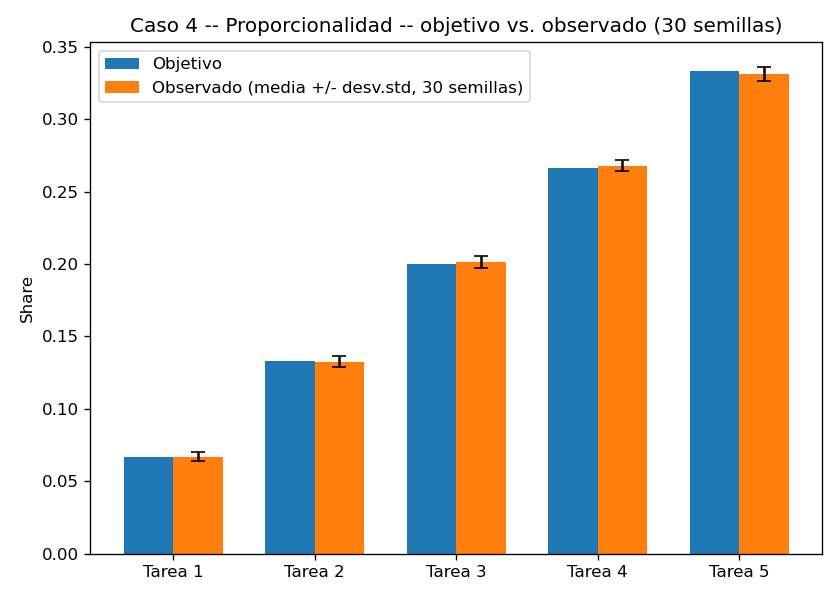
\includegraphics[width=\linewidth]{../../results/proporcionalidad/caso4_objetivo_vs_observado.png}
\caption{Caso 4 (Proporcionalidad): share objetivo vs. promedio observado
por tarea, con desviación estándar entre las 30 semillas como barra de
error. Generado por \texttt{scripts/experimento\_proporcionalidad.py}.}
\label{fig:objetivo-observado}
\end{figure}

\subsection{Análisis 1: la lotería no garantiza exactitud en ventanas cortas}

La Fig.~\ref{fig:convergencia} muestra el share acumulado de cada tarea
después de cada despacho, de una semilla representativa (\texttt{seed=1}),
desde el despacho 1 hasta el 10\,000. En los primeros cientos de despachos
las cinco líneas oscilan con amplitud grande y hasta se cruzan entre sí ---
la tarea 4 (40 boletos, objetivo $0.267$) llega a tener share $=1.0$
inmediatamente después del primer despacho, porque con una sola muestra
quien gana tiene automáticamente el 100\,\% de lo acumulado hasta ese punto.
A partir de aproximadamente el despacho 2000, cada línea se aplana en una
banda angosta alrededor de su objetivo (línea punteada) y prácticamente no
se mueve más.

\begin{figure}[htbp]
\centering
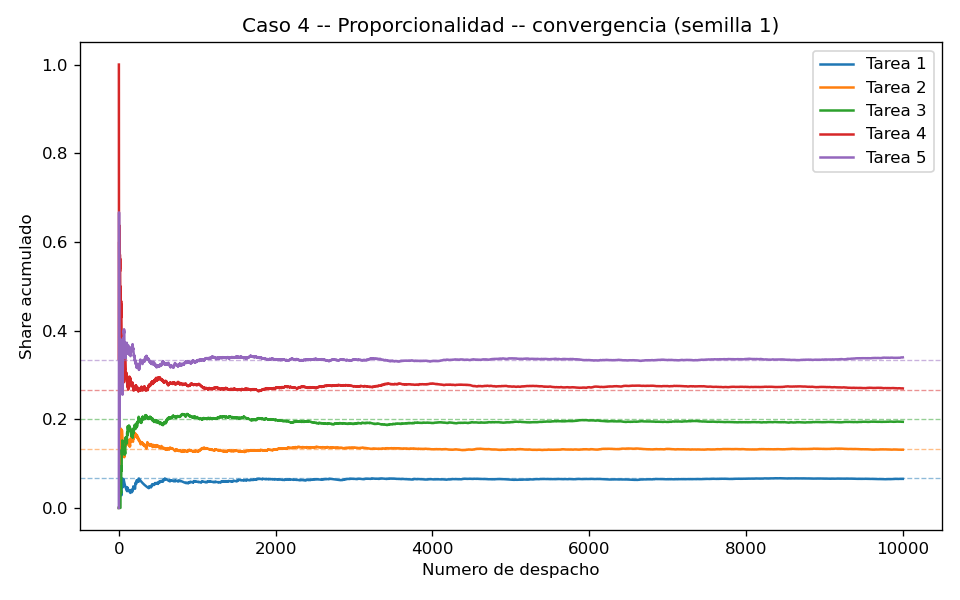
\includegraphics[width=\linewidth]{../../results/proporcionalidad/caso4_convergencia.png}
\caption{Caso 4: convergencia del share acumulado por tarea a lo largo de
$10^4$ despachos, semilla 1 (líneas punteadas: share objetivo de cada
tarea). El Caso 3 exhibe el mismo patrón hacia un único objetivo común de
$0.20$ (\texttt{results/proporcionalidad/caso3\_convergencia.png}).}
\label{fig:convergencia}
\end{figure}

La razón estructural: \texttt{observed\_share} de una tarea en el despacho
$k$ es un promedio acumulado (unidades corridas por esa tarea, dividido
entre unidades corridas por todas, hasta $k$). Un promedio de pocas
muestras está dominado por el resultado individual de esas muestras --- el
sorteo es \emph{correcto en expectativa} desde el primer despacho (cada
tirada respeta la ponderación de boletos, Sección~\ref{sec:analisis-extension}),
pero el \emph{promedio observado} de pocas tiradas no tiene por qué
parecerse todavía a esa expectativa: hace falta volumen para que el ruido
de tiradas individuales se cancele entre sí.

\subsection{Análisis 2: la variación cae como $1/\sqrt{N}$ con el número de despachos}

Se corrió el mismo Caso 4 (30 semillas) variando \texttt{--max-dispatches},
para medir cómo cae la desviación estándar (promediada entre las 5 tareas)
a medida que crece la ventana observada (Tabla~\ref{tab:ventana}).

\begin{table}[htbp]
\caption{Caso 4: error y desviación estándar según el tamaño de la ventana}
\label{tab:ventana}
\centering
\begin{tabular}{ccc}
\toprule
Ventana (despachos) & Error absoluto medio & Desv. estándar media \\
\midrule
50    & 0.006400 & 0.055580 \\
100   & 0.004800 & 0.037241 \\
500   & 0.001653 & 0.017224 \\
1000  & 0.001680 & 0.011512 \\
2500  & 0.001365 & 0.007220 \\
5000  & 0.001205 & 0.005499 \\
10000 & 0.001104 & 0.003978 \\
\bottomrule
\end{tabular}
\end{table}

La desviación estándar cae de $0.0556$ a $0.0040$ al pasar de 50 a 10\,000
despachos (ventana 200 veces más grande) --- una reducción de
\textbf{13.97 veces}, prácticamente idéntica a $\sqrt{200} \approx 14.14$.
Esto confirma que la variación entre semillas cae como $1/\sqrt{N}$ con el
número de despachos $N$: cada despacho adicional es, a efectos de esta
métrica, una observación más que se promedia con las anteriores, y el error
estándar de un promedio de $N$ observaciones aproximadamente independientes
escala como $1/\sqrt{N}$~\cite{NIST2003Handbook, NISTCSRCCLT}. Es el mismo
patrón de raíz cuadrada inversa
documentado para el número de \emph{semillas} en el experimento de la
extensión (Sección~\ref{sec:resultados-extension}) --- dos palancas
relacionadas pero no intercambiables: más despachos reduce el ruido de la
métrica dentro de una semilla; más semillas reduce la incertidumbre sobre
la media de una métrica ya ruidosa por semilla.

\subsection{Análisis 3: comparar shares entre tareas que terminan en momentos distintos puede engañar}

\texttt{observed\_share} se calcula sobre el total de unidades corridas por
\emph{todas} las tareas durante la ventana completa, lo que asume
implícitamente que todas siguen compitiendo durante toda la ventana. Si una
tarea termina su trabajo a mitad de camino y las demás siguen corriendo, el
denominador sigue creciendo con el trabajo de las tareas restantes mientras
el numerador de la que ya terminó queda fijo --- su share final calculado
sobre toda la ventana queda artificialmente bajo, no porque el sorteo la
haya tratado injustamente mientras competía, sino porque se le compara
contra unidades corridas después de que dejó de competir. Es exactamente
la razón por la que los Casos 3 y 4 usan tareas de $10^7$ unidades cada
una: con \texttt{--max-dispatches}$\,{=}\,10^4$ y quantum $1000$, el trabajo
total que cabe en la ventana está topado en $10^4 \times 1000 = 10^7$
unidades combinadas entre las 5 tareas --- muy por debajo de lo que
necesitaría cualquiera para agotar sus $10^7$ unidades individuales, así
que ninguna termina dentro de la ventana y todas compiten en igualdad de
condiciones. El Caso 5 (Terminación) usa deliberadamente lo contrario
--- trabajos de tamaños distintos --- pero por eso mismo no es un caso
válido para medir proporcionalidad por share acumulado: sirve para
verificar terminación correcta, no para comparar tasas de servicio entre
tareas que dejan de competir en momentos distintos.

Los resultados del experimento propio de la extensión (\textit{compensation
tickets}) se presentan junto con su diseño e hipótesis en la
Sección~\ref{sec:resultados-extension}, dentro de la Sección de Extensión,
en vez de aquí: a diferencia de este experimento de proporcionalidad (que
exige directamente el enunciado sobre el planificador base), ese es un
experimento A/B propio del equipo, y su resultado solo tiene sentido después
de conocer el mecanismo y las hipótesis H0/H1 que lo motivan.

\section{Extensión: Compensation Tickets}
\label{sec:extension}

\subsection{Extensión elegida y motivación}

De las cinco extensiones propuestas por el enunciado (Tabla~\ref{tab:opciones},
Sección~\ref{sec:analisis-extension}), el equipo eligió la
\textbf{Opción A: \textit{compensation tickets}}. La extensión exige
"modelar una tarea que cede antes de consumir el \textit{quantum} e inflar
temporalmente su valor según la fracción consumida", y responde a la
pregunta "¿recupera la participación de CPU a la que tenía derecho?". En el
paper original~\cite{Waldspurger1994}, este mecanismo compensa a un
servidor que se bloquea esperando E/S en nombre de un cliente y no debería
ser penalizado frente a clientes que nunca se bloquean: al reactivarse, el
servidor recibe temporalmente más boletos, proporcionales al inverso de la
fracción de su último \textit{quantum} que efectivamente usó, hasta agotar
el equivalente a un \textit{quantum} completo de CPU recibido en boletos
compensados.

Se eligió esta opción sobre las otras cuatro porque reutiliza el mismo
mecanismo cooperativo/quantum que el proyecto base de todas formas debía
implementar (no agrega una máquina de estados nueva ni una fuente de
eventos externa), porque su pregunta de evaluación se responde con el mismo
experimento de proporcionalidad que ya exige el proyecto (comparar
\texttt{observed\_share} con y sin compensación), y porque presenta menor
superficie de bugs de concurrencia nuevos que la Opción C (estados
cliente/servidor) o la D (doble contabilidad de monedas).

\subsection{El escenario debe forzarse}

Con el diseño base del planificador (modos cooperativo y quantum tal como
los especifica el enunciado), una tarea \emph{siempre} consume todo su
bloque asignado --- no existe ningún mecanismo para que ceda antes de
tiempo por cuenta propia. El escenario de cesión temprana que la extensión
necesita observar no puede surgir orgánicamente; hay que modelarlo
explícitamente, como pide el propio enunciado. Para eso se agregó un
parámetro opcional y exclusivo del experimento de la extensión:
\texttt{--yield-config <csv>}, un archivo con encabezado
\texttt{task\_id,yield\_percent} que le indica a tareas puntuales que cedan
tras correr solo una fracción de su bloque en vez de agotarlo. Ausente por
defecto, no tiene ningún efecto sobre los siete casos mínimos del
enunciado ni sobre el comportamiento base del planificador.

\subsection{Mecanismo}

El \textit{quantum} (o el bloque cooperativo) se mantiene fijo: lo que se
infla temporalmente son los \textbf{boletos} de la tarea que cedió temprano,
para darle mayor probabilidad de ganar los siguientes sorteos y así
compensar el turno reducido. Si una tarea consumió solo una fracción $f$ de
su bloque antes de ceder:
\begin{equation}
\text{tickets\_compensados} = \left\lceil \text{tickets\_base} \times \frac{1}{f} \right\rceil
\label{eq:compensacion}
\end{equation}
La compensación no es permanente: se mantiene mientras la tarea tenga una
\textbf{deuda} pendiente, definida como lo que le faltó para completar el
bloque original en la activación donde cedió. Cada vez que la tarea gana un
sorteo con boletos inflados, corre el bloque completo (ya no vuelve a ceder
mientras compensa) y descuenta lo corrido de la deuda; al llegar la deuda a
cero, \texttt{effective\_tickets} vuelve a \texttt{tickets\_base} y el ciclo
puede repetirse en la siguiente activación que gane.

\subsection{Decisiones de implementación}

Tres puntos que el diseño original dejaba abiertos a propósito se
resolvieron al implementar (detalle completo en
\texttt{decisiones\_diseno.md}, D15, del repositorio de conocimiento):

\begin{enumerate}
\item \textbf{La fracción $f$ se mide contra el bloque que decide el modo,
  no contra un quantum fijo.} Con dos modos de ejecución, $f$ se generaliza
  como $\text{unidades\_corridas} / \text{bloque\_decidido}$, donde
  \texttt{bloque\_decidido} es la misma cantidad que ya calculaba
  \texttt{decide\_slice\_units} para esa activación (quantum fijo, o el
  bloque cooperativo recortado por lo que falta) --- sin ramas de código por
  modo dentro de la extensión.
\item \textbf{El campo \texttt{tickets} de \texttt{Task} no se renombra.}
  Ya cumple el rol de "boletos base"; se agregó \texttt{effective\_tickets}
  como campo nuevo (igual a \texttt{tickets} salvo compensación activa) en
  vez de tocar los sitios que ya construían o leían \texttt{Task.tickets}
  desde el Milestone 1.
\item \textbf{La configuración de qué tareas ceden vive en un archivo
  aparte.} Nunca en el CSV principal de tareas: una bandera ausente por
  defecto es una garantía más fuerte de que los casos base no se ven
  afectados que una columna opcional que el parser tendría que aprender a
  ignorar.
\end{enumerate}

El control del experimento A/B (aislar el efecto de \emph{ceder} del efecto
de \emph{compensar}) tampoco estaba resuelto por el documento de diseño
original: se agregó \texttt{--disable-compensation}, que requiere
\texttt{--yield-config} y mantiene la cesión temprana activa pero nunca
infla \texttt{effective\_tickets} ---la tarea cede la misma fracción en cada
activación, indefinidamente, sin compensación--- de modo que la comparación
entre corridas con y sin esta bandera aísla exactamente el efecto de la
compensación en sí.

\subsection{Hipótesis}

\begin{itemize}
\item \textbf{H1.} Una tarea que cede voluntariamente antes de agotar su
  bloque, y que recibe \textit{compensation tickets} proporcionales a la
  fracción no consumida, alcanza un \texttt{observed\_share} significativamente
  más cercano a su share objetivo que la misma tarea bajo idénticas
  condiciones sin compensación.
\item \textbf{H0.} La compensación no tiene efecto medible sobre el
  \texttt{observed\_share} de una tarea que cede tempranamente.
\end{itemize}

El diseño experimental (control \texttt{--disable-compensation} vs.
tratamiento con compensación activa, misma semilla, mismo CSV, misma
ventana de despachos, repetido sobre múltiples semillas) y sus resultados
se presentan en la Sección~\ref{sec:resultados-extension}.

\section{Análisis del Paper}
\label{sec:analisis-extension}

\subsection{Problema y solución}

Waldspurger y Weihl~\cite{Waldspurger1994} identifican que los mecanismos de
planificación basados en prioridades (incluyendo esquemas de prioridad
dinámica como el de Unix) no ofrecen un control \emph{proporcional} y
predecible sobre la asignación de recursos: ajustar prioridades es una
operación ad-hoc, sin una relación cuantitativa clara entre el valor
asignado y la fracción de recurso efectivamente recibida, y las políticas
que sí intentan dar garantías proporcionales (como \textit{fair-share
scheduling} clásico) suelen requerir mecanismos de retroalimentación
complejos o no componen bien cuando los derechos deben transferirse
temporalmente entre entidades (por ejemplo, de un cliente bloqueado a un
servidor que trabaja en su nombre).

La solución propuesta es la \textbf{planificación por lotería}: cada
entidad recibe una cantidad de \textit{boletos} que representa su derecho
sobre el recurso, y cada decisión de asignación se resuelve sorteando un
boleto al azar entre los boletos activos. El mecanismo es simple de
implementar, componible (los boletos se pueden agrupar, transferir o
subdividir sin lógica especial), y --- a diferencia de los esquemas de
prioridad --- da una garantía \emph{probabilística} de proporcionalidad en
vez de una garantía determinista de corto plazo.

\subsection{Proporcionalidad probabilística}

La proporcionalidad de la lotería es un resultado esperado, no una garantía
por despacho: cada sorteo es un ensayo de Bernoulli independiente, y la
fracción de sorteos ganados por una tarea con $t_i$ boletos de un total
activo $T$ converge a $t_i/T$ por la ley de los grandes números conforme
aumenta el número de sorteos observados, con una varianza que decrece con
ese mismo número~\cite{NIST2003Handbook, Illowsky2024}. Es exactamente lo
que exhibe la Fig.~\ref{fig:convergencia}
(Sección~\ref{sec:resultados}): en pocos cientos de despachos el share
observado todavía oscila con amplitud visible; hacia el final de la ventana
de $10^4$ despachos converge de forma estable a la fracción objetivo. Este
carácter probabilístico --- y no una asignación exacta y determinista de
cada intervalo --- es la diferencia conceptual central entre la
planificación por lotería y un planificador de cuotas fijas.

\subsection{Extensión elegida frente a las demás opciones}

El enunciado ofrece cinco extensiones posibles sobre el mecanismo base
(Tabla~\ref{tab:opciones}); el equipo eligió la Opción A
(\textit{compensation tickets}, Sección~\ref{sec:extension}) por las razones
ya expuestas: reutiliza el mecanismo cooperativo/quantum que el proyecto
base debía implementar de todas formas, y su pregunta de evaluación se
responde con el mismo experimento de proporcionalidad que ya exige el
proyecto.

\begin{table}[htbp]
\caption{Las 5 extensiones propuestas por el enunciado}
\label{tab:opciones}
\renewcommand{\arraystretch}{1.25}
\begin{tabular}{p{1.6cm}p{2.7cm}}
\toprule
\textbf{Opción} & \textbf{Requisito mínimo} \\
\midrule
A. \textit{Compensation tickets} (elegida) & Modelar una tarea que cede antes del quantum e inflar temporalmente su valor \\
\midrule
B. Boletos dinámicos & Aplicar cambios de tickets en despachos definidos por un archivo de eventos \\
\midrule
C. \textit{Ticket transfer} & Modelar cliente bloqueado y servidor que recibe temporalmente sus boletos \\
\midrule
D. \textit{Currencies} & Dos monedas respaldadas por shares base e inflación local \\
\midrule
E. Selección $O(\log n)$ & Árbol de sumas parciales en vez de lista acumulativa \\
\bottomrule
\end{tabular}
\end{table}

Las opciones descartadas se evaluaron y se prefirió A sobre ellas por menor
superficie de bugs de concurrencia nuevos: C requiere modelar estados
cliente/servidor adicionales a los tres estados de \texttt{Task} ya
definidos; D requiere una doble contabilidad de monedas con su propia
lógica de conversión; B modifica la asignación de boletos desde una fuente
externa durante la corrida, lo que interactúa con la validación de entrada
de formas que el enunciado no especifica. E se discute también en la
Sección~\ref{sec:tradeoffs} como \textit{trade-off} de diseño, ya que su
pregunta de evaluación (¿en qué tamaño de carga compensa la complejidad
$O(\log n)$?) es ortogonal a la elegida y aplica independientemente de qué
extensión funcional se implemente.

\subsection{Diferencias con la implementación sobre Mach 3.0}

El paper original valida \textit{lottery scheduling} integrándolo al
planificador de hilos del \textbf{microkernel Mach 3.0}, reemplazando su
política de prioridades sobre hardware y cargas de trabajo reales: hilos
del kernel, interrupciones de temporizador reales que disparan la
expropiación, bloqueo real en E/S, y múltiples tipos de recurso
(incluyendo memoria y ancho de banda de red) generalizados bajo el mismo
mecanismo de boletos.

Este proyecto es, por diseño, una \textbf{simulación en espacio de
usuario}: no se modifica el \textit{kernel} ni se sustituye el planificador
real de GNU/Linux, que sigue decidiendo los ciclos de CPU físicos por
debajo sin que el programa lo sepa. Las diferencias concretas son:

\begin{itemize}
\item \textbf{Un único CPU lógico simulado}, aplicado mediante el
  protocolo de mutex/condvars de la Sección~\ref{sec:arquitectura}, en vez
  de la expropiación real por interrupción de temporizador del kernel.
\item \textbf{Carga de trabajo sintética e instrumentada} (la serie de
  Taylor de $\pi$) en vez de cargas de programas reales; se eligió
  precisamente porque su estado es verificable, no porque modele algo del
  mundo real.
\item \textbf{Un único tipo de recurso} (unidades de CPU lógicas), sin la
  generalización a memoria o ancho de banda que el paper demuestra.
\item \textbf{Sin cesión real por E/S}: la cesión temprana de la extensión
  se fuerza explícitamente vía \texttt{--yield-config} en vez de surgir de
  un bloqueo de E/S real, porque el prototipo no tiene E/S que modelar.
\end{itemize}

\subsection{Limitaciones del prototipo}

Además de las diferencias estructurales con Mach 3.0, el prototipo tiene
limitaciones propias de su alcance como proyecto de curso: opera sobre un
conjunto fijo de tareas conocido de antemano en el CSV de entrada (el paper
soporta creación dinámica de hilos con boletos heredados); el rango de 5 a
25 tareas es una cota de validación del enunciado, no una limitación
inherente del mecanismo de lotería; la selección de la ganadora es
$O(n)$ sobre la lista de tareas activas (Opción E, no implementada,
discutida como \textit{trade-off} en la Sección~\ref{sec:tradeoffs}); y no
se implementa \textit{ticket transfer} (Opción C), por lo que el prototipo
no demuestra directamente el mecanismo que el paper usa para resolver
inversión de prioridad en llamadas cliente-servidor --- solo su analogía
más cercana, la compensación por cesión temprana.

\section{Discusión de \textit{Trade-offs}}
\label{sec:tradeoffs}

\subsection{Quantum fijo vs. bloque proporcional: costo de coordinación}

Los modos cooperativo y quantum son mecánicamente idénticos --- comparten
el mismo bucle del worker (Algoritmo~\ref{alg:worker}) y la misma función de
ejecución; solo difiere cómo se calcula el tamaño del bloque por activación
(Sección~\ref{sec:algoritmos}). Esa única diferencia tiene, sin embargo, un
costo de coordinación medible y opuesto según el tamaño relativo de las
tareas. Con quantum fijo $Q$, una tarea pequeña frente a $Q$ puede terminar
en una sola activación mientras una tarea grande necesita muchas; con un
bloque proporcional al tamaño de cada tarea, todas necesitan
aproximadamente el mismo número de activaciones sin importar su
\texttt{work\_units} total, a costa de que una tarea grande ceda el CPU con
más frecuencia de la que cedería bajo un quantum fijo equivalente. El Caso~6
del enunciado lo hace explícito con una sola tarea de 60 unidades: al 10\,\%
cooperativo (bloques de 6) necesita 10 activaciones; con quantum $Q=25$
(bloques 25+25+10) necesita solo 3, para exactamente el mismo trabajo total
y el mismo resultado de $\pi$. Más activaciones significan más ciclos de
mutex/condvar y más filas de log por unidad de trabajo real completada ---
el \textit{overhead} de coordinación del protocolo de la
Sección~\ref{sec:protocolo}, que no aparece en el resultado final observable
pero sí en el costo de producirlo.

\subsection{Reproducibilidad vs. realismo temporal}

El enunciado exige que la misma entrada, semilla, modo y parámetros
produzcan exactamente el mismo registro de decisiones (determinismo). Esto
se logra midiendo el trabajo en \texttt{work\_units} lógicas --- iteraciones
discretas de la serie de $\pi$ --- en vez de tiempo real de CPU, y usando
aritmética entera (Algoritmo~\ref{alg:cooperativo}) en vez de \texttt{double}
para el cálculo del bloque cooperativo, evitando que la representación de
punto flotante introduzca variación entre corridas idénticas por diferencias
de redondeo entre plataformas. El costo de esa reproducibilidad es
\textbf{realismo}: en un sistema real, el tiempo que una tarea recibe
depende de interrupciones de temporizador, latencia de memoria, otros
procesos del sistema operativo real corriendo por debajo, y variabilidad de
\textit{hardware} --- ninguno de esos factores está presente aquí. La
elección es deliberada y coherente con el objetivo del proyecto (verificar
un protocolo de sincronización y una política de asignación, no medir
rendimiento real de un sistema), pero implica que los números de
\textit{overhead} de coordinación de la sección anterior son comparables
\emph{entre sí} (mismo entorno lógico) y no directamente extrapolables al
costo real de cambio de contexto de un \textit{scheduler} de producción.

\subsection{Selección $O(n)$ por lista vs. árbol de sumas parciales $O(\log n)$}

El sorteo (Algoritmo~\ref{alg:sorteo}) localiza a la ganadora recorriendo la
lista de tareas \texttt{READY} y acumulando boletos hasta que el boleto
sorteado cae en el rango de alguna --- costo $O(n)$ por despacho, donde $n$
es el número de tareas activas. La Opción E del enunciado
(Tabla~\ref{tab:opciones}) propone sustituir esa lista por un árbol de sumas
parciales, reduciendo la localización a $O(\log n)$. Para el rango de
tareas que exige este proyecto (5 a 25), la diferencia entre $O(n)$ y
$O(\log n)$ es de a lo sumo un factor de $25/\log_2 25 \approx 5$
comparaciones por despacho --- indistinguible en la práctica frente al costo
fijo de las dos llamadas a \texttt{pthread\_mutex\_lock}/\texttt{unlock} y
la señal de condvar que rodean cada sorteo. La complejidad adicional de
mantener un árbol balanceado (actualizar sumas parciales cada vez que una
tarea cambia de estado o de boletos efectivos, en vez de solo recorrer un
arreglo) solo se justificaría con cientos o miles de tareas activas
simultáneas, un régimen muy distinto al de este proyecto; de ahí que se
prefiriera reutilizar el mecanismo cooperativo/quantum (Opción A) en vez de
optimizar una operación que no es el cuello de botella real a esta escala.

\subsection{Equidad de corto plazo vs. largo plazo}

La proporcionalidad de la lotería es, por diseño, una propiedad de largo
plazo (Sección~\ref{sec:analisis-extension}): si una corrida se deja
avanzar hasta que todas las tareas terminan, \texttt{observed\_share}
converge a $1/N$ para todas, sin importar sus boletos, simplemente porque
cada tarea termina consumiendo exactamente su trabajo total y las que
tienen más boletos solo llegan ahí más rápido. La ponderación real por
boletos únicamente es observable dentro de una \textbf{ventana truncada}
(\texttt{--max-dispatches}) sobre trabajo suficientemente grande, como en
los Casos 3 y 4 (Sección~\ref{sec:resultados}). Esto implica un
\textit{trade-off} de medición, no solo de diseño: la elección del tamaño de
la ventana observada determina qué se puede concluir sobre equidad ---una
ventana demasiado corta introduce más varianza de corto plazo (menos
sorteos acumulados para que la ley de los grandes números converja);
demasiado larga, y algunas tareas empiezan a terminar, sesgando el share de
las que quedan. La elección de ventana usada en los Casos 3/4 de este
informe ($10^4$ despachos sobre tareas de $10^7$ unidades) se validó
verificando que ninguna tarea llega a completar su trabajo dentro de la
ventana (Sección~\ref{sec:resultados}); la sensibilidad de este mismo
\textit{trade-off} es aún más pronunciada al medir el efecto de la
extensión de compensación, cuyo análisis de robustez frente al tamaño de
ventana está en elaboración (Sección~\ref{sec:resultados-extension}).

\section{Conclusiones}

El planificador implementado traduce la política de \textit{proportional-share
scheduling} de Waldspurger y Weihl a un mecanismo ejecutable y verificable en
espacio de usuario, cumpliendo las restricciones de concurrencia del
enunciado: exclusión mutua verificada en tiempo de ejecución (el
\texttt{assert} de \texttt{sync\_dispatch}), sin espera activa (todo bloqueo
pasa por variables de condición con predicado explícito), y sin un único
candado que envuelva la ejecución del trabajo real. Los siete casos mínimos
de funcionamiento cumplen, verificados bajo AddressSanitizer,
UndefinedBehaviorSanitizer, LeakSanitizer y ThreadSanitizer sin hallazgos, y
el experimento de proporcionalidad confirma que el sorteo pondera
correctamente por boletos dentro de una ventana de observación truncada,
con error absoluto medio muy por debajo de la tolerancia exigida.

La extensión elegida, \textit{compensation tickets}, reutiliza el mecanismo
cooperativo/quantum ya construido para modelar una tarea que cede
tempranamente y recupera participación de CPU mediante boletos inflados
temporalmente, sin alterar el comportamiento del planificador base cuando la
extensión no está activa. La cuantificación estadística final de cuánta
participación recupera --- y su sensibilidad al tamaño de la ventana
observada --- se completa en la Sección~\ref{sec:resultados-extension}.

La comparación con el paper original deja claras las simplificaciones
deliberadas de este prototipo: un único CPU lógico simulado en vez de
integración real con un \textit{kernel}, una carga de trabajo sintética e
instrumentada en vez de programas reales, y un único tipo de recurso en vez
de la generalización a memoria y red que demuestra Mach 3.0. Estas
simplificaciones son coherentes con el objetivo del proyecto --- verificar
el protocolo de sincronización y la política de asignación, no medir
rendimiento de un sistema real --- y se documentan explícitamente en vez de
presentarse como limitaciones no reconocidas.

\section*{Declaración de Transparencia, Uso de IA y Material Reutilizado}

Para la redacción de este informe se utilizó Claude Code (Anthropic) como
herramienta auxiliar de apoyo: síntesis de las decisiones de diseño y
hallazgos técnicos ya documentados por el equipo a lo largo del proyecto,
redacción del texto en español, generación del pseudocódigo y las figuras a
partir del código fuente real y de los datos experimentales reproducidos
para este documento, y revisión ortográfica y de formato. Todo el contenido
técnico (arquitectura, algoritmos, resultados de pruebas y experimentos) se
verificó contra el código fuente y las corridas reales del programa antes
de incluirse.

Fuera de la plantilla LaTeX \texttt{IEEEtran} (uso académico estándar, bajo
su propia licencia) y la cita al paper original de Waldspurger y
Weihl~\cite{Waldspurger1994}, este informe y el código del proyecto no
reutilizan material de terceros: todo el código fuente, pseudocódigo,
figuras y datos experimentales fueron producidos por el equipo
específicamente para este proyecto.


% ===================
% References
% ===================
\bibliographystyle{IEEEtran}
\bibliography{referencias}

\end{document}
